\documentclass[8.5pt,twoside,twocolumn]{article}
\oddsidemargin -1.2cm
\evensidemargin -1.2cm
\textwidth 18cm
\headheight 1.0in
\topmargin -3.5cm
\textheight 22cm
\usepackage[super,sort&compress,comma]{natbib} 
%\usepackage{mhchem}
\usepackage{amsmath}
\usepackage{times,mathptmx}
% \usepackage{times}
% feel free not to use mathptmx if it causes difficulties
\usepackage{sectsty}
\usepackage{balance} 

\usepackage{graphicx} %eps figures can be used instead
\usepackage{lastpage}
\usepackage[format=plain,justification=raggedright,singlelinecheck=false,font=small,labelfont=bf,labelsep=space]{caption} 
\usepackage{fancyhdr}
\pagestyle{fancy}

\usepackage{SIunits}

\usepackage{pgfplots}
\usepgfplotslibrary{external}
\usepgfplotslibrary{groupplots}
\usetikzlibrary{positioning}
\usetikzlibrary{plotmarks}
\usetikzlibrary{patterns}
\tikzexternalize
\tikzsetexternalprefix{fig_}
\tikzset{external/force remake}
\tikzset{every mark/.append style={scale=0.8}}
\pgfplotsset{every axis/.append style={small}}

\begin{document}

\thispagestyle{plain}
\fancypagestyle{plain}{
\fancyhead[L]{
\includegraphics[height=8pt]{headers/LH}}
\fancyhead[C]{\hspace{-1cm}
\includegraphics[height=20pt]{headers/CH}}
\fancyhead[R]{
\includegraphics[height=10pt]{headers/RH}\vspace{-0.2cm}}
\renewcommand{\headrulewidth}{1pt}}
\renewcommand{\thefootnote}{\fnsymbol{footnote}}
\renewcommand\footnoterule{\vspace*{1pt}% 
\hrule width 3.4in height 0.4pt \vspace*{5pt}} 
\setcounter{secnumdepth}{5}



\makeatletter 
\def\subsubsection{\@startsection{subsubsection}{3}{10pt}{-1.25ex plus -1ex minus -.1ex}{0ex plus 0ex}{\normalsize\bf}} 
\def\paragraph{\@startsection{paragraph}{4}{10pt}{-1.25ex plus -1ex minus -.1ex}{0ex plus 0ex}{\normalsize\textit}} 
\renewcommand\@biblabel[1]{#1}            
\renewcommand\@makefntext[1]% 
{\noindent\makebox[0pt][r]{\@thefnmark\,}#1}
\makeatother 
\renewcommand{\figurename}{\small{Fig.}~}
\sectionfont{\large}
\subsectionfont{\normalsize} 

\fancyfoot{}
\fancyfoot[LO,RE]{\vspace{-7pt}
\includegraphics[height=9pt]{headers/LF}}
\fancyfoot[CO]{\vspace{-7.2pt}\hspace{12.2cm}
\includegraphics{headers/RF}}
\fancyfoot[CE]{\vspace{-7.5pt}\hspace{-13.5cm}
\includegraphics{headers/RF}}
\fancyfoot[RO]{\footnotesize{\sffamily{1--\pageref{LastPage} ~\textbar  \hspace{2pt}\thepage}}}
\fancyfoot[LE]{\footnotesize{\sffamily{\thepage~\textbar\hspace{3.45cm} 1--\pageref{LastPage}}}}
\fancyhead{}
\renewcommand{\headrulewidth}{1pt} 
\renewcommand{\footrulewidth}{1pt}
\setlength{\arrayrulewidth}{1pt}
\setlength{\columnsep}{6.5mm}
\setlength\bibsep{1pt}

\twocolumn[
  \begin{@twocolumnfalse}
\noindent\LARGE{\textbf{Quantitative localisation and sizing of polydisperse colloids from confocal microscopy images}}
\vspace{0.6cm}

\noindent\large{\textbf{Mathieu Leocmach\textit{$^{a}$} and
Hajime Tanaka$^{\ast}$\textit{$^{a}$}}}\vspace{0.5cm}
%Please note that \ast indicates the corresponding author(s) but no footnote text is required. 


\noindent\textit{\small{\textbf{Received Xth XXXXXXXXXX 20XX, Accepted Xth XXXXXXXXX 20XX\newline
First published on the web Xth XXXXXXXXXX 200X}}}

\noindent \textbf{\small{DOI: 10.1039/b000000x}}
\vspace{0.6cm}
%Please do not change this text.

\vspace{0.5cm}
 \end{@twocolumnfalse}
  ]

\tikzset{external/force remake=false}
\tikzsetnextfilename{localise}
\begin{figure*}
	\centering
	\begin{tikzpicture}[
		pic3d/.style={inner sep=0}, %
		lab/.style={above right, text height=0.8em, text depth=0.2em, font=\Large\bfseries}%
		]%
		\node[pic3d] (m3d) {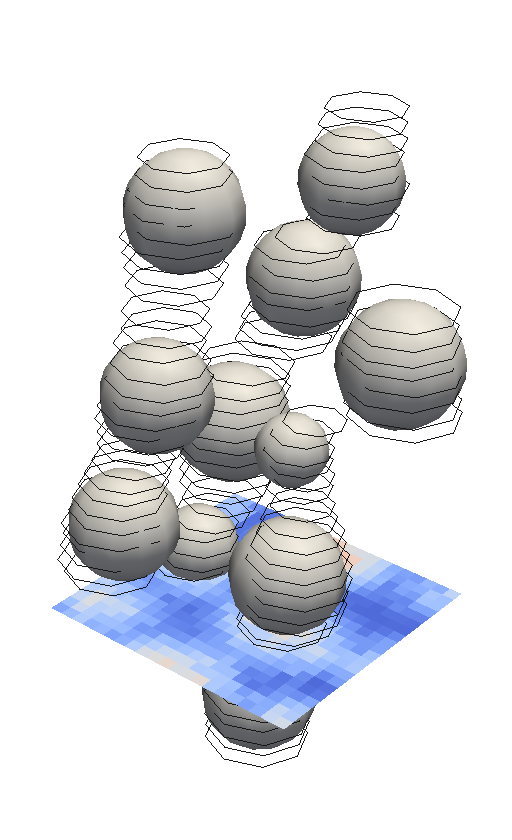
\includegraphics[width=0.28\textwidth]{comp2D3D_crop}};
		\node[lab] at (m3d.south west) {a};
		\node [pic3d, right] at (m3d.east) (m2d) {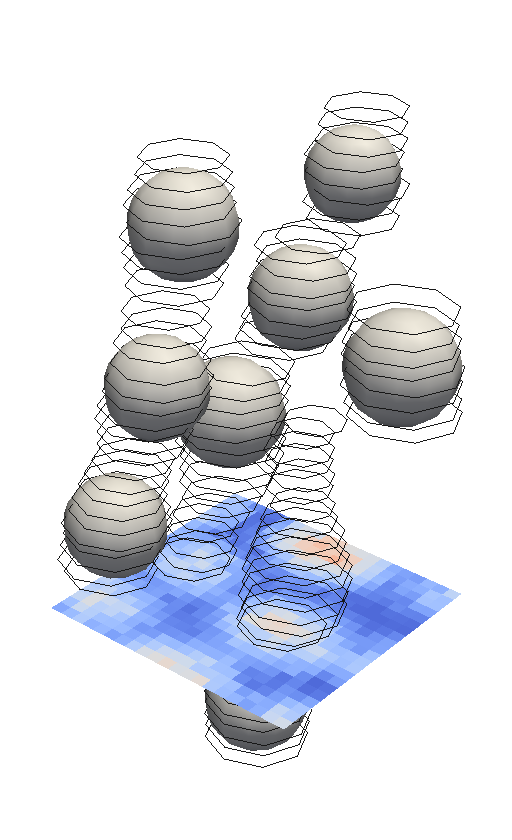
\includegraphics[width=0.28\textwidth]{comp2D_reconstructed_crop}};
		\node[lab] at (m2d.south west) {b};
		\node [pic3d, below right] at (m2d.north east) (cg20) {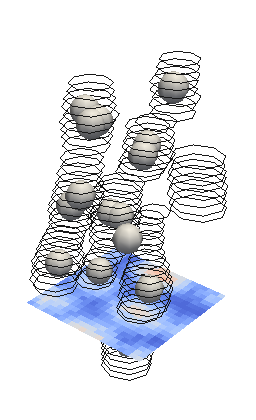
\includegraphics[width=0.14\textwidth]{comp3D_monoscale_r20_crop}};
		\node[lab] at (cg20.south west) {c};
		\node [pic3d, right] at (cg20.east) (cg25) {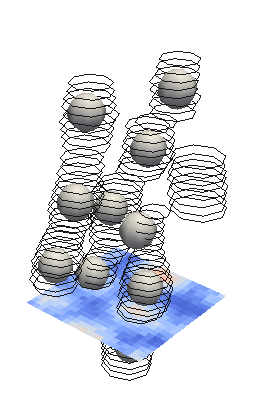
\includegraphics[width=0.14\textwidth]{comp3D_monoscale_r25_crop}};
		\node[lab] at (cg25.south west) {d};
		\node [pic3d, right] at (cg25.east) (cg30) {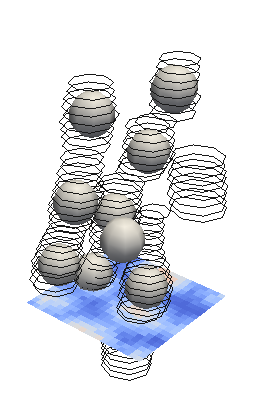
\includegraphics[width=0.14\textwidth]{comp3D_monoscale_r30_crop}};
		\node[lab] at (cg30.south west) {e};
		\node [pic3d, above right] at (m2d.south east) (cg35) {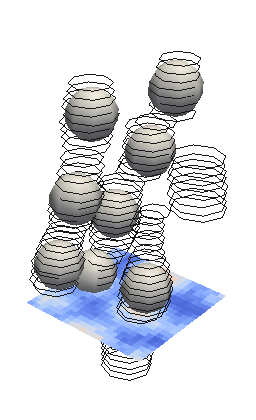
\includegraphics[width=0.14\textwidth]{comp3D_monoscale_r35_crop}};
		\node[lab] at (cg35.south west) {f};
		\node [pic3d, right] at (cg35.east) (cg40) {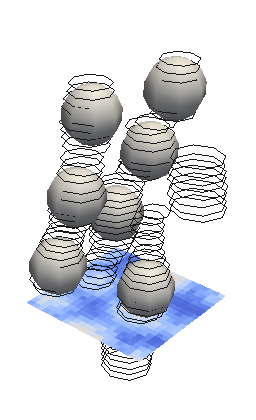
\includegraphics[width=0.14\textwidth]{comp3D_monoscale_r40_crop}};
		\node[lab] at (cg40.south west) {g};
		\node [pic3d, right] at (cg40.east) (cg45) {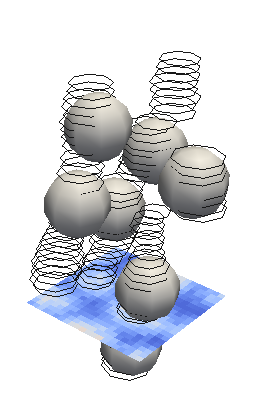
\includegraphics[width=0.14\textwidth]{comp3D_monoscale_r45_crop}};
		\node[lab] at (cg45.south west) {h};
	\end{tikzpicture}
	\caption{\textbf{Visualisation of the results of various tracking methods for the same portion of image.} \textbf{a} Multiscale 3D tracking. \textbf{b} Reconstruction from 2D tracking. \textbf{c-h} Crocker and Grier in 3D with blurring radius increasing from \unit{2}{px} to \unit{4.5}{px} by steps of \unit{0.5}{px}. The circles on each picture are the result of 2D multiscale tracking of each XY slice of the 3D pictures. Sphere are displayed with radii determined by the tracking methods in \textbf{a-b}, and equal to the blurring radius for \textbf{c-h}.}
	\label{fig:localise}
\end{figure*}

\tikzset{external/force remake}
\tikzsetnextfilename{sizing}
\begin{figure}
	\centering
	\begin{tikzpicture}[lab/.style={above left, text height=0.8em, text depth=0.2em, font=\Large\bfseries}]
	\begin{axis}[%
		name=hist,
		width=0.6\columnwidth, height=0.6\columnwidth,%
		%scale only axis,
		xmin=1, xmax=5,
		axis y line*=left,
		ymin=0, ytick=\empty,%
		ylabel={Size distribution (a.u.)},%
		ylabel near ticks,
		]
		\addplot[ybar, ybar interval] file {SEM_size_distrib.txt};
	\end{axis}
	\begin{axis}[%
		%scale only axis,
		width=0.6\columnwidth, height=0.6\columnwidth,%
		xmin=1, xmax=5,
		axis y line*=right,
		xlabel={Diameters [$\micro\metre$]},%
		ymin=0, ytick=\empty,%
		no marks,%
		]
		\addplot+[dashed] file {go1_intensity.sizes};
		\addplot table [x expr ={\thisrowno{0}/1.23}, y index=1] {go1_intensity.sizes};
		\draw[->, ultra thick] (axis cs:3.15,0.05) -- (axis cs: 3.9, 0.05);% node[right)] {swelling};
		\node[lab] at (rel axis cs:0.95,0.95) {a};
	\end{axis}
	\begin{axis}[%
		at={(0.55\columnwidth,0)},
		width=0.5\columnwidth, height=0.6\columnwidth,%
		xmin=0, xmax=1.5,%
		xlabel ={$r/\left\langle \sigma\right\rangle$, $\hat{r}$},%
		ymin=0,%
		ylabel=$g(r)$, ylabel near ticks,%
		no marks,%
		legend style={legend pos=north west}
		]
		\addplot+[dashed] table [x expr ={\thisrowno{0}/13}, y index=1] {go1.rdf};
		\addplot table [x expr ={\thisrowno{0}/0.9096}, y expr={\thisrowno{1}*7.5}] {go1.srdf};
		\legend{$g(r)$, $g(\hat{r})$};
		\node[lab] at (rel axis cs:0.95,0.95) {b};
	\end{axis}
	\end{tikzpicture}
	\caption{\textbf{Sizing} of our colloids. \textbf{a} Size distribution estimated \emph{in situ} (dashed line) by our multiscale algorithm ($\sim 1.8\times 10^6$ instantaneous sizing). Comparison with the size distribution estimated from scanning electron microscopy of only $140$ dry particles (steps) is possible once controlled for $23\%$ of swelling (full line). A careful comparison between confocal images and algorithm output suggest that the thick tail of small particles is not an artefact, thus the relative lack of small particles in the SEM measurement is probably due to bad sampling. \textbf{b} First peak of the radial distribution function with (full line) and without (dashed) the size data. Taking into account the measured sizes rectifies the effect of the polydispersity: the peak is thinner and higher.}
	\label{fig:sizing}
\end{figure}


\tikzset{external/force remake=false}
\tikzsetnextfilename{deconv}
\begin{figure}
	\centering
	\begin{tikzpicture}[
		lab/.style={above right, text height=0.8em, text depth=0.2em, font=\Large\bfseries}%
		]%
		\begin{groupplot}[%
		group style={
				group name=pics,
				group size=2 by 2,%
				horizontal sep=0.0075\textwidth,
				vertical sep=0.0075\textwidth,
				},%
		width=0.225\textwidth,%
		height=0.2475\textwidth,%
		xmin=0,xmax=50,ymin=0,ymax=55,%
		axis lines=none,%
		scale only axis=true,%
		point meta=explicit symbolic,%
		scatter/@pre marker code/.code={%
        	\pgfmathparse{10*\pgfplotspointmetatransformed*\pgfplotsunitxlength}%
        	%\pgfplotstransformcoordinatex{\pgfplotspointmetatransformed}
            \def\markopts{mark=o,black,mark size=\pgfmathresult}%
            \expandafter\scope\expandafter[\markopts]
            },%
        scatter/@post marker code/.code={\endscope} 
		]
		\nextgroupplot
			\addplot graphics [xmin=0,xmax=50,ymin=0,ymax=55]{Zelong_original};
			\node[lab] at (rel axis cs:0,0){a};
		\nextgroupplot
			\addplot graphics [xmin=0,xmax=50,ymin=0,ymax=55]{Zelong_blurred};
			\addplot+[only marks, scatter] table [x index=1, y expr={55-\thisrowno{2}}, meta index=3] {Z_elong.xyz};
			\node[lab] at (rel axis cs:0,0){b};
		\nextgroupplot
			\addplot graphics [xmin=0,xmax=50,ymin=0,ymax=55]{Zelong_deconvolved};
			\addplot+[only marks, scatter] table [x index=1, y expr={55-\thisrowno{2}}, meta index=3] {Z_elong_deconv.xyz};
			\node[lab] at (rel axis cs:0,0){c};
		\nextgroupplot
			\node[lab] at (rel axis cs:0,0){d};
		\end{groupplot}
		\begin{axis}[%
			at={(pics c2r2.south west)},%
			anchor=outer south west,
			width=0.225\textwidth,%
			height=0.28\textwidth,%
			xlabel = {$r$ [$\micro\metre$]}, ylabel={$g(r)$},%
			xlabel near ticks, ylabel near ticks,
			xmin=0,xmax=4,ymin=0,%
			no marks,%
			]
			\addplot file {cp0.34.rdf};
			\addplot file {cp0.34_deconv.rdf};
		\end{axis}
	\end{tikzpicture}
	\caption{\textbf{Deconvolution.} Detail of the same $YZ$ slice of \textbf{a} original confocal image, \textbf{b} previous blurred by $\sigma_0=1.6$, \textbf{c} previous deconvolved by measured kernel (see text). Circles indicate the tracked particles position and size when using whether \textbf{b} or \textbf{c} as first Gaussian layer $G_0$. All three centres are in the slice $\pm \unit{0.5}{px}$. \textbf{d} Radial distribution function of sticky spheres (blue) without and (red) with deconvolution.}
	\label{fig:deconv}
\end{figure}


\tikzset{external/force remake=false}
\tikzsetnextfilename{perfect}
\begin{figure*}
	\centering
	\begin{tikzpicture}[
		lab/.style={above right, text height=0.8em, text depth=0.2em, font=\Large\bfseries}%
		]%
	\pgfplotsset{cycle list name=black white}
	\begin{axis}[%
		name=errorsize,
		width=0.45\textwidth,%
		xlabel={Input radius (px)}, ylabel={Radius relative error (\%)},%
		extra x ticks={3.47}, extra x tick labels={}, extra tick style={grid=major},%
		extra y ticks={0}, extra y tick labels={}
		]
		\addplot table [x index=0, y expr ={100*(\thisrowno{1}/\thisrowno{0}-1)}] {multiscale_relative_sizes.out};
		\node[lab] at (rel axis cs:0,0) {a};
	\end{axis}
		
	\begin{axis}[%
		xlabel near ticks,ylabel near ticks,
		tiny,
		width=0.25\textwidth,%
		at=(errorsize.north east),	anchor=north east,%
		xlabel={Input radius}, ylabel={Output radius},%
		extra x ticks={3.47}, extra x tick labels={}, extra tick style={grid=major},%
		ytick={2,4,...,14},
		axis background/.style={fill=white},%
		]
		\addplot+[only marks, mark size=0.5, mark=o] table [x index=0, y expr ={\thisrowno{1}}] {multiscale_relative_sizes.out};
		\addplot+[no marks, domain=1.5:14] {x};
	\end{axis}
	
	\begin{axis}[%
		at={(0.5\textwidth,0)},%
		width=0.45\textwidth,%
		xlabel={$r_{ij}$ (px)}, ylabel={$r_{ij}$ error (\unit{0.01}{px})},%
		xmin=8, xmax=18,%
		extra tick style={grid=major},%
		extra y ticks={0}, extra y tick labels={}
		]
		\addplot table [x index=0, y expr ={(\thisrowno{2}-\thisrowno{1}-\thisrowno{0})*100}] {close_neighbours3D.out};
		\draw (axis cs:12,-6) circle[radius=0.03\textwidth] (axis cs:16,-6) circle[radius=0.03\textwidth];
		\draw[dashed] (axis cs:12,-6) -- (axis cs:12,-8) (axis cs:16,-8) -- (axis cs:16,-6);
		\draw[<->] (axis cs:12,-8) -- (axis cs:16,-8) node[midway, below] {$r_{ij}$};
		\draw[->] (axis cs:12,-4) -- +(0.03\textwidth,0) node[midway, above] {\unit{4}{px}};
		\draw[->] (axis cs:16,-4) -- +(-0.03\textwidth,0) node[midway, above] {\unit{4}{px}};
		\draw[->, very thick] (axis cs:16,-6) -- (axis cs:14,-6);
		\node[lab] at (rel axis cs:0,0) {b};
	\end{axis}
	
	\begin{axis}[%
		at={(0.5\textwidth,-0.4\textwidth)},%
		width=0.45\textwidth,%
		xlabel={$r_{ij}$ (px)}, ylabel={$R$ (px)},%
		xmin=8, xmax=18,%
		extra tick style={grid=major},%
		extra y ticks={4}, extra y tick labels={},%
		legend style={legend pos=south east}
		]
		\addplot table [x index=0, y index=4] {close_neighbours3D.out};
		\addplot+[mark=square] table [x index=0,y index=6] {close_neighbours3D.out};
		\legend{No correction, One iteration};
		\node[lab] at (rel axis cs:0,0) {c};
	\end{axis}
	
	\begin{axis}[%
		at={(0,-0.4\textwidth)},%
		width=0.45\textwidth,%
		area legend,
		const plot, no marks,%
		xlabel={$R$ (px)}, ylabel={Size distribution},%
		%xmin=8, xmax=18,%
		extra tick style={grid=major},%
		extra x ticks={5.298}, extra x tick labels={},%
		ymin=0,%		
		legend style={legend pos=north west, cells={anchor=west}}
		]
		\addplot+[pattern=north west lines] file {john_exact_mono_large_init.hist} \closedcycle;
		\addplot+[gray, fill=gray, semitransparent] file {john_exact_mono_large_cor1.hist} \closedcycle;
		\addplot+[pattern=dots] file {john_exact_mono_large_cor2.hist};
		\legend{No correction, One iteration, Two iterations};
		\draw[decorate,decoration=brace] (axis cs:4.75, 200) -- (axis cs:5.05, 200) node[midway, above] {edges};
		\node[lab] at (rel axis cs:0,0) {d};
	\end{axis}
	\end{tikzpicture}
	\caption{\textbf{Results from perfect images.} \textbf{a} Sizing of an isolated sphere. Left of the vertical line our algorithm uses a doubled image. \textbf{b} Localisation error and \textbf{c} sizing error function of the distance between two particles. Oscillations are due to off-lattice centre position. \textbf{d} Size distribution extracted from digitized configuration of 4000 monodisperse hard spheres at $0.50$ volume fraction (vertical line indicates the input radius). The tail to the right is due to particles on the edges of the image who have fewer neighbours and thus are more `dilute'. \textbf{c} and \textbf{d} also show the effect of finite dilution correction up to convergence.}
	\label{fig:perfect}
\end{figure*}

\end{document}